\documentclass[student]{ITRslides}
\usepackage{tikz,pgfplots}
\addbibresource{ref.bib}
\graphicspath{{pics/}{logos/}}

\title{Control of a multi-robot cooperative team guided by a human operator}
\presenter{M. Angerer}

\supervisor{S. Musi\'c}
\typeofpres{Intermediate Presentation Master Thesis}

\usetikzlibrary{decorations.pathreplacing}
\newcommand{\tikzmark}[2]{\tikz[remember picture,baseline=(#1.base)]{\node[inner sep=0pt] (#1) {#2};}}
%%%%%%%%%%%%%%%%%%%%%%%%%%%%%%%%%%%%%%%%%%%%%%%%%%%%%%%%%%%%%%%%%%%%%%%%%%%%%%%%

\begin{document}


\begin{frame}
    \titlepage
\end{frame}

%\begin{frame}
%	\frametitle{Overview}
%    \tableofcontents%[hideallsubsections]%[pausesections]
%\end{frame}

\section{Introduction}

\begin{frame}
	\frametitle{Why use cooperative manipulation with human guidance?}
		\begin{columns}[t]
		\column{0.55\linewidth}
	
			\begin{figure}
			\centering
			%\psfrag{q1}[Bl][Bl]{\small $\alpha$}
			\includegraphics[width=0.98\textwidth]{mhi-meister45.jpg}
			\caption{Coordinated handling of tools by a tele-operated robot \cite{MHI-MEISTeR}}
			\end{figure}
		
		\column{0.55\linewidth}
			
		Human reasoning
		\begin{itemize}
			\item Foresight and adaptiveness to incidents
			\item Superior planning capabilities
		\end{itemize}
		Enhanced flexibility of multiple robots
			\begin{itemize}
				\item Transportation of large/heavy objects
	\item Assembly of multiple parts 
	\item Coordinated use of tools
			\end{itemize}
			
			\end{columns}
\end{frame}

\begin{frame}
	\frametitle{Problem Formulation}

	\begin{itemize}
		\item Precise and stable control during free-motion/contact transition
		\item Enhance versatility by performing friction grasps
		\item (Intuitive) high-level human supervisory control
		\item Local formation constraints controlled by robots
		\item Assistance of the operator with suitable feedback
	\end{itemize}

\end{frame}

\begin{frame}
	\frametitle{Related Work: Robot-team control}
	\begin{itemize}
		\item Formation control of robot team \cite{Sieber_15,Wimboeck_06}
		\begin{itemize}
			\item object not part of control loop
			%\item no knowledge of object required
		\end{itemize}
		\item Intrinsically Passive Control \cite{Stramigioli_01, Wimboeck_08}
		\begin{itemize}
			\item virtual object simulation
			%\item knowledge of object shape and dynamics required
		\end{itemize}
		\item Internal impedance control + object dynamics' feed-forward \cite{DePascali_15}
				\begin{itemize}
			\item object tracking required
			%\item knowledge of object shape and dynamics required
		\end{itemize}
		\item Internal and external impedance control \cite{Caccavale_01,Caccavale_08}
			\begin{itemize}
			%\item object tracking required
			%\item knowledge of object shape and dynamics required
			\item Force/Torque sensors at the manipulators required
			\end{itemize}
	\end{itemize}
\end{frame}

\begin{frame}
	\frametitle{Related Work: Human in the loop}
	\begin{itemize}
		\item Bilateral tele-manipulation  \cite{Lee_05}
		\begin{itemize}
			\item Single master, constrained system as slave
			\item Local control of interaction dynamics
			\item Force feedback
		\end{itemize}
		\item Formation-based shared control \cite{Sieber_15, Scheggi_14}
		\begin{itemize}
			\item Single leader, multiple followers
			\item Robots preserve formation autonomously
			\item Tactile feedback
		\end{itemize}
		\item Gesture Control \cite{Gioioso_2014}
		\begin{itemize}
			\item Hand motion controls constrained system
			\item Hand pose controls grasping process
			%\item only visual feedback
		\end{itemize}
		\end{itemize}
\end{frame}

\section{Approach}

\begin{frame}
	\frametitle{Energy consistent modelling and control}
	\begin{itemize}
		\item \emph{Virtual object} concept
			\begin{itemize}%[leftmargin=0em]
  				\renewcommand{\labelitemi}{$\Rightarrow$}
				\item Maps object forces to manipulators
				\item Stores kinetic energy
				\item Changes size to adjust formation
			\end{itemize}
		\item Controller represents energy content of the complete system
		\item Dampers dissipate energy: \textbf{passive system}
		\item Operator controls system by energy  supply
		\item Model errors never influence passivity nor stability
		\end{itemize}
%\begin{itemize}%[leftmargin=0em]
%  \renewcommand{\labelitemi}{$\Rightarrow$}
%\item enhanced human perception through control of a meaningful quantity and appropriate feedback
%\item stability over a wide class of environments
%			\end{itemize}
%		\begin{quote}
%		If a controlled robot is not passive there is always a passive environment that destabilizes the interconnected system \cite{Stramigioli_15}
%		\end{quote}


\end{frame}
\begin{frame}
	\frametitle{System modelling}
	\textit{How can we consistently model different forms of energy stored in a system?\\}
	\textbf{Port-Hamiltonian systems\\}
	\begin{itemize}
	
		\item Mechanical elements
			\begin{itemize}
			\item \tikzmark{L}{Spring \;\;\;}
			\item Mass
			\item \tikzmark{I}{Damper}
			\end{itemize}
			\begin{tikzpicture}[remember picture,overlay]
    \draw[decorate,decoration={brace}] (L.north east) -- node[right] {Impedance control components} (L.north east |- I.south east);
\end{tikzpicture}
		\item Conservative elements
			\begin{itemize}
			\item Transformer
			\item Gyrator
			\end{itemize}
			\item Interconnection through power ports
		\[ \mathcal{P} = \mathcal{V} \times \mathcal{V}^* \]
%		\item Example: variable rest-length spring
%		\begin{eqnarray}\label{EQ:variablerestlengthspring}
%	\dot{H}_i^j =\left( \begin{pmatrix}1 & Ad_{H_b^j}\end{pmatrix} \begin{pmatrix}T_b^{j} \\ T_i^{b}\end{pmatrix} \right) H_i^j\\
%	\begin{pmatrix}W_b^{j,j} \\ W_i^{b,b}\end{pmatrix}  = \left( \begin{pmatrix}1 \\ Ad_{H_b^j}^T\end{pmatrix} \frac{\partial V_{i,j}}{\partial H_i^j} \right) (H_i^j)^T
%\end{eqnarray}

\end{itemize}

\end{frame}

%\begin{frame}
%	\frametitle{Intrinsically Passive Control (IPC)}
%	\begin{columns}
%		\column{0.4\linewidth}
%			
%	
%		\begin{itemize}
%			\item High-level Supervisor and low-level IPC
%			\item IPC + robot: passive
%			\item Power provided by Supervisor
%			\item Environment assumed passive
%		\end{itemize}
%
%		
%		\column{0.58\linewidth}
%             \begin{figure}[htb]
%			\centering
%			%\psfrag{q1}[Bl][Bl]{\small $\alpha$}
%			\includegraphics[width=0.9\textwidth]{IPCoverview.png}
%			\caption{Overview of the IPC architecture 								\cite{Stramigioli_01}}
%			\end{figure}
%		
%			
%		\end{columns}
%\end{frame}

\begin{frame}
	\frametitle{Intrinsically Passive Control}
\begin{columns}[t]
		\column{0.5\linewidth}
			
	
		\begin{itemize}
			\item Geometric interconnection of springs, masses and dampers
			\item Internal and external \emph{impedance} relations
			\item No manipulator inertia re-shaping
			\item Energy supplied by operator/environment
			\item Grasping with variable rest-length springs
		\end{itemize}

		
		\column{0.5\linewidth}
             \begin{figure}[htb]
			\centering
			%\psfrag{q1}[Bl][Bl]{\small $\alpha$}
			\includegraphics[width=0.98\textwidth]{IPCsprings.png}
			\caption{Mass-spring-damper structure of the IPC 						\cite{Stramigioli_01}}
			\end{figure}
		
			
		\end{columns}
\end{frame}

%\begin{frame}
%	\frametitle{Grasping an object}
%\begin{columns}
%		\column{0.4\linewidth}
%			
%	
%		\begin{itemize}
%			\item Variable rest-length springs
%			\item Rest-length: virtual object size
%			\item Distinct power port
%		\end{itemize}
%
%		
%		\column{0.62\linewidth}
%             \begin{figure}[htb]
%			\centering
%			%\psfrag{q1}[Bl][Bl]{\small $\alpha$}
%			\includegraphics[width=0.98\textwidth]{IPCobjects.png}
%			\caption{Virtual and real object \cite{Wimboeck_08}}
%			\end{figure}
%		
%			
%		\end{columns}
%\end{frame}

\begin{frame}
	\frametitle{Human supervisory control}
	\begin{itemize}
			\item Command value: velocity $\Leftrightarrow$ force :feedback value
			\item Suitable for bilateral tele-manipulation
			\item Energy intuition: humans can estimate possible impacts of interaction
			\item Spring rest-lengths: adjust to grasp/release objects
		\end{itemize}
\end{frame}


\section{Results}
%\begin{frame}
%	\frametitle{Grasping force optimization for friction contacts}
%	\begin{columns}
%	\column{0.6\textwidth}
%	\begin{itemize}
%	\item required contact normal force is dependent on tangential forces
%	\item high tangential forces arise during acceleration
%	\item other requirements: safety margin, maximum grasping force $\Rightarrow$ cost function
%	\item linear matrix inequality (LMI) problem
%	\end{itemize}
%	\column{0.5\textwidth}
%
%\begin{figure}[htb]
%			\centering
%			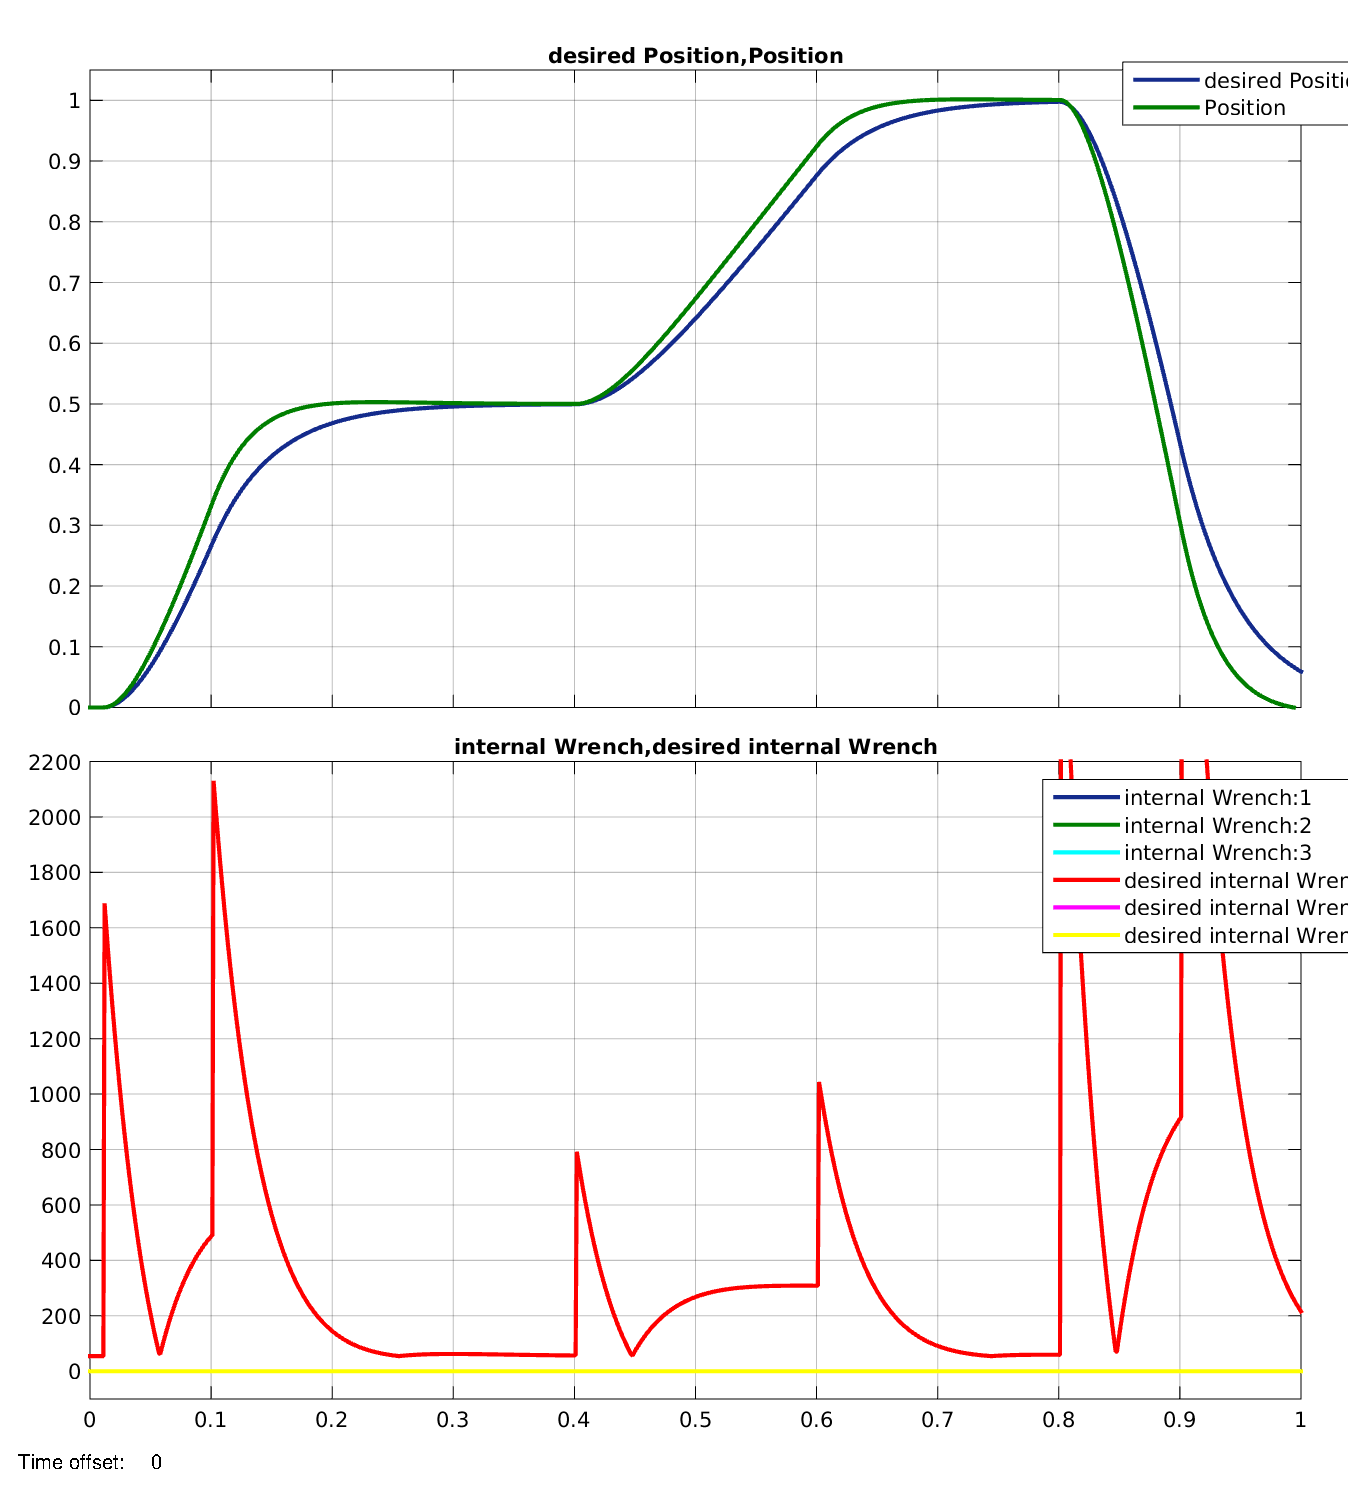
\includegraphics[width=0.9\textwidth]{Hanposforce.eps}
%			\caption{Position, Internal wrench}
%\end{figure}
%\end{columns}
%\end{frame}
\begin{frame}
	\frametitle{Comparison: position tracking}
%Impedance-based reference trajectory generation \cite{Caccavale_01}
\begin{figure}[t]
\begin{tikzpicture}
	\begin{axis} [
		ylabel = {$p_x$[m]},
		xlabel = {t[s]},
		minor y tick num = 1,
		axis lines = left,
		legend entries = {position, desired position},
		legend style = {at={(axis cs:2.5, 0.7)}, anchor = north},
		legend cell align=left,
		grid = major,
		height=3.5cm,
		width=0.98\linewidth
	]
\addplot[red,]
	table {/home/mangerer/MAgit/MA/Latex/plotdata/DePatransPosition.txt};
\addplot[blue,]
	table {/home/mangerer/MAgit/MA/Latex/plotdata/DePatransdesiredPosition.txt};
%\draw[->, thick] (axis cs:5, 10) -- (axis cs:7, 9);
%\draw[->, thick] (axis cs:15, 8) -- (axis cs:13.3, 6);
%\draw[<->, thick] (axis cs:5.35, 5) -- (axis cs:5.35, 17);
%\node at (axis cs:2.5,11){\small{\parbox{3.2cm}{Increased internal stress for $N_{h} \neq \{ 1{,}2{,}3\}$} }};
%\node at (axis cs:15.5,9){\small{Placeholder}};
\end{axis}
\end{tikzpicture}
\begin{tikzpicture}
	\begin{axis} [
		ylabel = {$p_x$[m]},
		xlabel = {t[s]},
		minor y tick num = 1,
		axis lines = left,
		legend entries = {position,desired position},
		legend style = {at={(axis cs:2.6, 0.7)}, anchor = north},
		legend cell align=left,
		grid = major,
		height=3.5cm,
		width=0.98\linewidth
	]
\addplot[red,]
	table {/home/mangerer/MAgit/MA/Latex/plotdata/DIPCtransPosition.txt};
\addplot[blue,]
	table {/home/mangerer/MAgit/MA/Latex/plotdata/DIPCtransdesiredPosition.txt};
\end{axis}
\end{tikzpicture}
\vspace{-20pt}
\caption{Top: Object force feed-forward;
Bottom: Virtual Object}
\end{figure}
\end{frame}

\begin{frame}
	\frametitle{Comparison: velocity tracking}
%Internal impedance control with object force-feedforward \cite{DePascali_15}
\begin{figure}[t]
\begin{tikzpicture}
	\begin{axis} [
		ylabel = {$v_x$[m/s]},
		xlabel = {t[s]},
		minor y tick num = 1,
		axis lines = left,
		legend entries = {velocity, desired velocity},
		legend style = {at={(axis cs:0.8, -0.5)}, anchor = north},
		legend cell align=left,
		grid = major,
		height=3.5cm,
		width=0.98\linewidth
	]
\addplot[red,]
	table {/home/mangerer/MAgit/MA/Latex/plotdata/CaVi_Velocity.txt};
\addplot[blue,]
	table {/home/mangerer/MAgit/MA/Latex/plotdata/CaVi_desiredVelocity.txt};
\end{axis}
\end{tikzpicture}
\begin{tikzpicture}
	\begin{axis} [
		ylabel = {$v_x$[m]},
		xlabel = {t[s]},
		minor y tick num = 1,
		axis lines = left,
		legend entries = {velocity,desired velocity},
		legend style = {at={(axis cs:0.8, -0.5)}, anchor = north},
		legend cell align=left,
		grid = major,
		height=3.5cm,
		width=0.98\linewidth
	]
\addplot[red,]
	table {/home/mangerer/MAgit/MA/Latex/plotdata/DIPCtransVelocity.txt};
\addplot[blue,]
	table {/home/mangerer/MAgit/MA/Latex/plotdata/DIPCtransdesiredVelocity.txt};
\end{axis}
\end{tikzpicture}
\vspace{-20pt}
\caption{Top: External impedance based reference trajectory generation; Bottom: Virtual object}
\end{figure}
\end{frame}

\begin{frame}
	\frametitle{Comparison: internal forces (rotation)}
\begin{figure}[t]

\begin{tikzpicture}
	\begin{axis} [
		ylabel = {f[N],m[Nm]},
		xlabel = {t[s]},
		minor y tick num = 1,
		axis lines = left,
		legend entries = {force $f_{int,x}$, force $f_{int,y}$, torque $m_{int,z}$},
		legend style = {at={(axis cs:2.6, 0.04)}, anchor = north},
		legend cell align=left,
		grid = major,
		height=3.3cm,
		width=0.98\linewidth
	]
\addplot[red,]
	table {/home/mangerer/MAgit/MA/Latex/plotdata/DePaIntWrenchtx.txt};
\addplot[blue,]
	table {/home/mangerer/MAgit/MA/Latex/plotdata/DePaIntWrenchty.txt};
	\addplot[green,]
	table {/home/mangerer/MAgit/MA/Latex/plotdata/DePaIntWrenchrz.txt};\end{axis}
\end{tikzpicture}
\begin{tikzpicture}
	\begin{axis} [
		ylabel = {f[N],m[Nm]},
		xlabel = {t[s]},
		minor y tick num = 1,
		axis lines = left,
		legend entries = {force $f_{int,x}$, force $f_{int,y}$, torque $m_{int,z}$},
		legend style = {at={(axis cs:2.6, 0.04)}, anchor = north},
		legend cell align=left,
		grid = major,
		height=3.3cm,
		width=0.98\linewidth
	]
\addplot[red,]
	table {/home/mangerer/MAgit/MA/Latex/plotdata/DIPCInternalWrenchtx.txt};
\addplot[blue,]
	table {/home/mangerer/MAgit/MA/Latex/plotdata/DIPCInternalWrenchty.txt};
	\addplot[green,]
	table {/home/mangerer/MAgit/MA/Latex/plotdata/DIPCInternalWrenchrz.txt};\end{axis}
\end{tikzpicture}
\vspace{-25pt}
\caption{Top: Object force feed-forward;
Bottom: Virtual Object}
\end{figure}
\end{frame}
\section{Conclusion}

\begin{frame}
	\frametitle{Conclusion}
	...
\end{frame}
\appendix
%\nocite{buss11}
%\nocite{bauer09}
\begin{frame}[allowframebreaks]
	\frametitle{References}
	%\tiny
	%\bibliographystyle{plain}
	%\bibliography{ref}
	\printbibliography
\end{frame}


\end{document}
